\subsubsection{Modelo denso}


Este modelo es un modelo con solo capas de tipo \textit{forward-pass}. Tiene otras dos capas pero que no implementan lógica asociada a lo que es la red neuronal en sí, sino que son capas de traducción de matriz a vector y viceversa como se explicará a continuación. Gráficamente la red que se ha definido es la siguiente:
\begin{figure}[H]
    \centering
    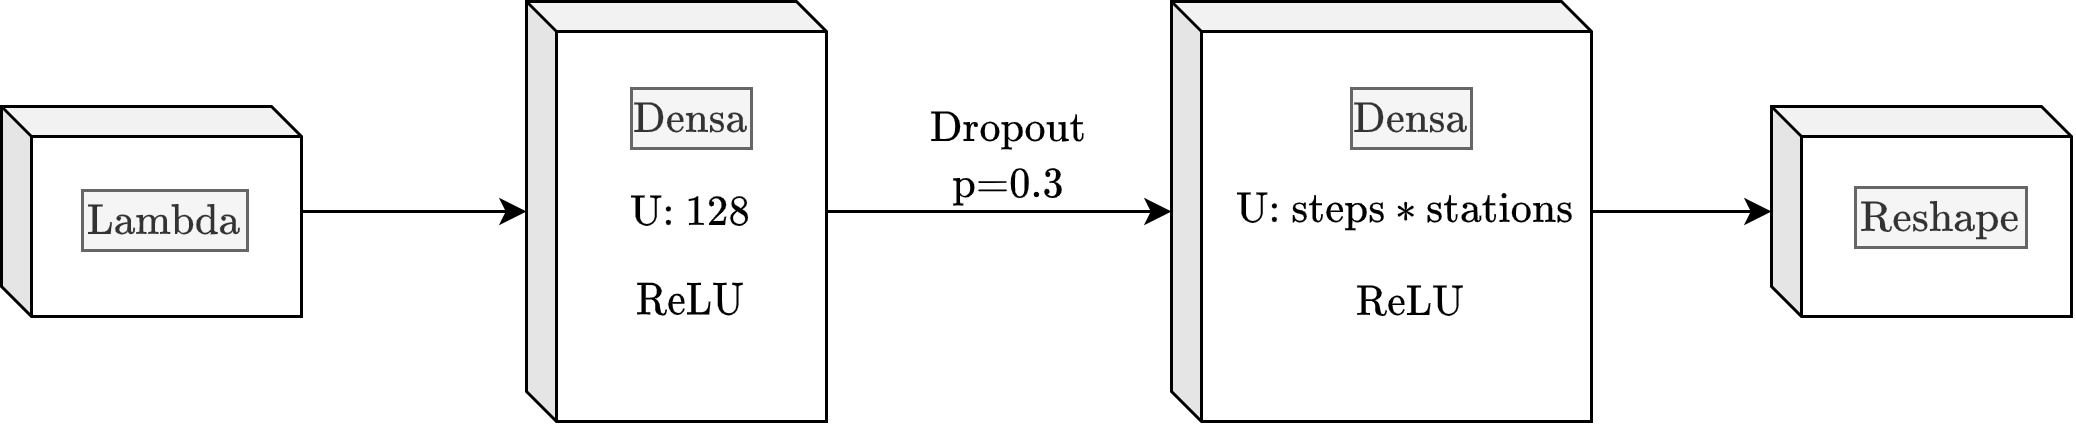
\includegraphics[width=12cm]{images/solution/models/dense.png}
    \caption{Modelo denso}
    \label{fig:dense-model}
\end{figure}

La primera capa oculta tiene $128$ unidades. La cantidad de capas y cantidad de neuronas que tiene una capa son parámetros que se han puesto de forma pseudoaleatoria. Se han realizado distintas combinaciones probando distintas cantidades de unidades y 2 capas densas con $128$ unidades en la primera es la combinación que mejores resultados ha obtenido. La segunda capa oculta tiene la misma cantidad de unidades que valores tiene que devolver el modelo, que es un valor calculado por la multiplicación entre el número de estaciones con las que se está trabajando, $633$, por el número de intervalos que se quieren calcular. Por ejemplo, si se quiere calcular un único intervalo para todas las estaciones, el vector de dicha capa será de $633$ elementos, si se quiere calcular dos intervalos, el número de elementos del vector será $1266 = 2 \times 633$ y así sucesivamente. Esta capa es común a todos los modelos que se explicarán de aquí en adelante.
\newline

La última capa es una capa de tipo \textit{Reshape}. Esta capa no tiene ni función de activación ni parámetros que ajustar porque lo único que hace es convertir el vector de la capa anterior a una matriz más comprensible y con la que se puede trabajar de forma más cómoda con el \textit{dataset} donde cada fila será un intervalo y cada columna será una estación. Los valores de esta matriz seránpor tanto la predicción que el modelo devuelve para el intervalo y estación definidas por su fila y columna en el que se encuentran.
\newline

Siguiendo la misma lógica, la primera capa es de tipo \textit{Lambda} y se encarga de realizar la tarea opuesta, dada una matriz obtener un vector. Las capas \textit{Lambda} son capas en las que el usuario define una función que se quiera ejecutar.
\newline

El código de este modelo se ha definido como se muestra a continuación:

\begin{minted}[fontsize=\scriptsize]{python}
from tensorflow.keras.models import Sequential
from tensorflow.keras.layers import Reshape, Dense, Dropout, Lambda

# `steps` is a variable which has the number of intervals to be predict
steps = 0 

# `stations` is the number of stations in the bike network
stations = 0

dense_model = Sequential([
    # Matrix to vector
    Lambda(lambda x: x[:, -1:, :]), 
    
    # Input layer
    Dense(128, activation="relu"),

    Dropout(0.3),
    
    # Ouput layer
    Dense(steps * stations),
                  
    # Vector to matrix
    Reshape([steps, stations])
])
\end{minted}


Los resultados del modelo se pueden ver junto al resto de resultados en la sección \ref{results}.